\documentclass{article}
\usepackage[utf8]{inputenc}
\usepackage[english]{babel}
\usepackage[T1]{fontenc}
\usepackage{amsmath,amssymb,amsfonts,amsthm}
\usepackage{ulem}
\usepackage{subcaption}
\usepackage{caption}
\usepackage{gauss}
\usepackage{mathtools}
\usepackage{mathrsfs}
\usepackage{hyperref}
\usepackage{bbm}
\usepackage{graphicx} 
\usepackage{enumerate} 
\usepackage{fancyhdr} 
\usepackage{lastpage} 
\usepackage[margin=1in,footskip=0.25in]{geometry}
\usepackage{pdfpages}
\usepackage{pdfpages}
\usepackage{bookmark}

\pagestyle{fancy}
\setcounter{MaxMatrixCols}{20}
\linespread{1,2}
\newcommand{\pic}[3]{\makebox[\textwidth]{\textbf{#1}}
\\
\begin{center}
\includegraphics[scale=#2,center]{#3}
\end{center}}
\newcommand{\QQ}{\mathbb{Q}}
\newcommand{\RR}{\mathbb{R}}
\newcommand{\BB}{\mathbb{B}}
\newcommand{\NN}{\mathbb{N}}
\newcommand{\FF}{\mathbb{F}}
\newcommand{\ZZ}{\mathbb{Z}}
\newcommand{\CC}{\mathbb{C}}
\newcommand{\EE}{\mathbb{E}}
\newcommand{\indi}[1]{\mathbbm{1}_{#1}}
\newcommand{\limi}[2]{\liminf\limits_{#1\rightarrow#2}}
\newcommand{\bcup}[1]{\bigcup\limits_{#1}}
\newcommand{\bcap}[1]{\bigcap\limits_{#1}}
\newcommand{\m}{\cdot}
\newcommand{\TF}[2]{\{#1_{#2}\}_{#2\in\mathbb{N}}}
\newcommand{\Ma}[2]{\left( \begin{array}{{#1}}
#2
\end{array} \right)}
\newcommand{\Mp}[1]{\begin{pmatrix}
    #1
    \end{pmatrix}}
\newcommand{\M}[1]{\begin{matrix}
    #1
    \end{matrix}}
\newcommand{\ver}[2]{#1\hspace{0.05cm}\vert\hspace{0.03cm}#2}
\newcommand{\mgd}[2]{\left\{#1 \hspace{0.1cm}\left|\hspace{0.1cm}#2\right.\right\}}
\newcommand{\llim}[2]{\lim\limits_{#1\rightarrow #2}}
\newcommand{\ls}{\limsup\limits_{n\rightarrow\infty}}
\newcommand{\li}{\liminf\limits_{n\rightarrow\infty}}
\newcommand{\Part}[2]{\frac{\partial{#1}}{\partial{#2}}}
\newcommand{\Int}[4][x]{\int_{#2}^{#3} #4 \hspace{0.05cm}\mathrm{d} #1}
\newcommand{\myeq}[2][=]{\mathrel{\overset{\makebox[0pt]{\mbox{\normalfont\tiny\sffamily $#2$}}}{#1}}}
\newcommand{\Myeq}[2][\leq]{\mathrel{\overset{\makebox[0pt]{\mbox{\normalfont\tiny\sffamily $#2$}}}{#1}}} 
\newcommand{\mb}[1]{\mathbb{#1}}
\newcommand{\mc}[1]{\mathcal{#1}}
\newcommand{\ms}[1]{\mathscr{#1}}
\newcommand{\as}{\myeq[\rightarrow]{as}}
\newcommand{\As}{\myeq[\sim]{as}}
\newcommand{\wk}{\myeq[\rightarrow]{wk}}
\newcommand{\Pkonv}{\myeq[\rightarrow]{P}}
\newcommand{\Dkonv}{\myeq[\rightarrow]{D}}
\newcommand{\Lkonv}[1][1]{\myeq[\rightarrow]{\mc{L}^{#1}}}
\newcommand{\borel}{\ms{B}(\mb{R})}
\newcommand{\inte}[3]{\int_{#1} #2 \hspace{0.05cm}\mathrm{d}{#3}}
\newcommand{\Norm}[1]{\left\lVert#1\right\rVert}
\newcommand{\norm}[1]{\left\lvert#1\right\rvert}
\newcommand{\Sum}[2]{\sum\limits_{#1}^{#2}}

\title{}
\author{}
\makeatletter
\providecommand*{\cupdot}{%
  \mathbin{%
    \mathpalette\@cupdot{}%
  }%
}
\newcommand*{\@cupdot}[2]{%
  \ooalign{%
    $\m@th#1\bigcup$\cr
    \hidewidth$\m@th#1\cdot$\hidewidth
  }%
}
\makeatother



\begin{document}

% import the frontpage
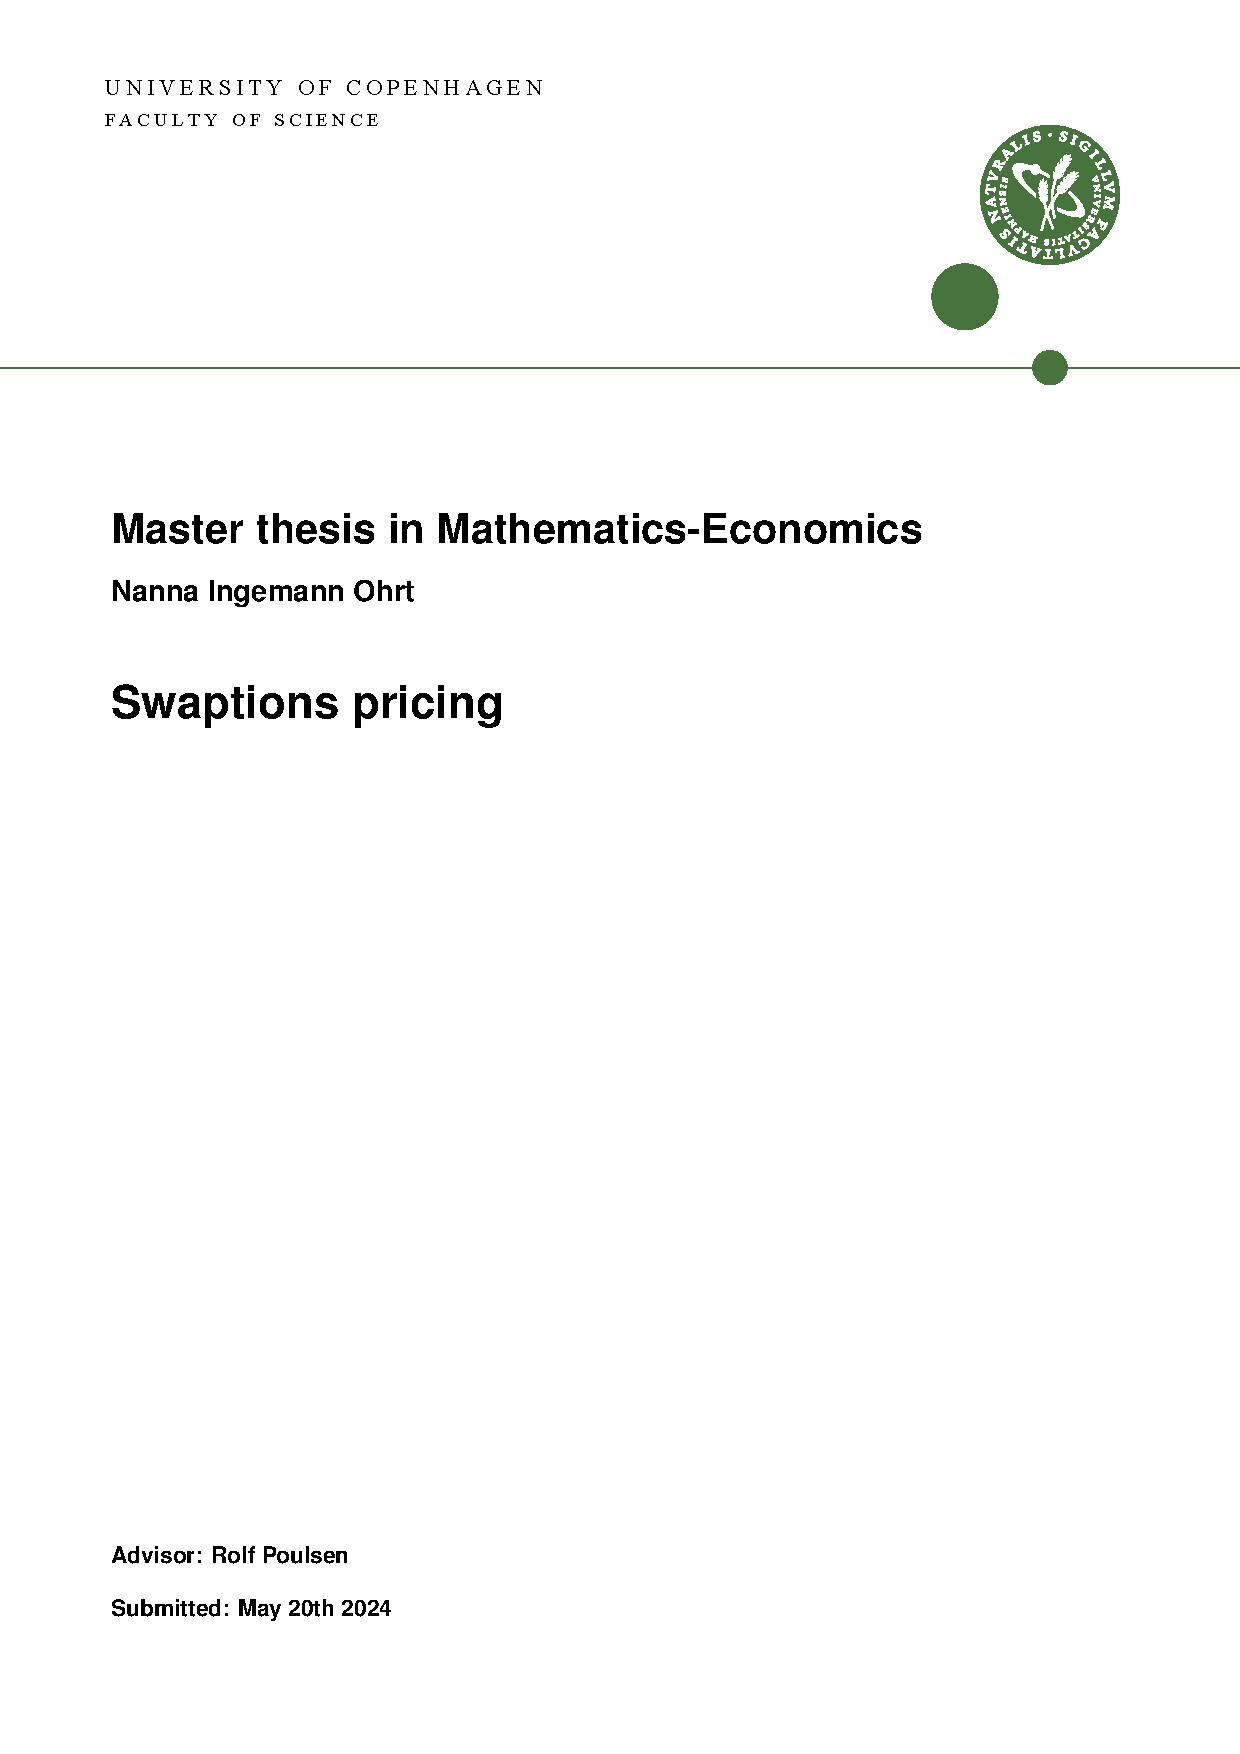
\includepdf[pages=-]{/Users/nannaingemannohrt/Desktop/master_thesis/frontpage/frontpage_setup.pdf}

\tableofcontents
\newpage

% import the introduction
\section{Introduction}




\begin{tikzpicture}[node distance=1cm and 1cm, auto]
  % Nodes
  \node (t0) {Time 0};
  \node[below= of t0] (t1) {Time 1};
  \node[below= of t1] (t2) {Time 2};
  \node[below= of t2] (t3) {Time 3};
  \node[below= of t3] (t4) {Time 4};
  
  % Arrows
  \draw[-Latex] (t0.south) to [bend right] node[left] {forward} (t1.north);
  \draw[-Latex] (t1.south) to [bend right] node[left] {forward} (t2.north);
  \draw[-Latex] (t2.south) to [bend right] node[left] {forward} (t3.north);
  \draw[-Latex] (t3.south) to [bend right] node[left] {forward} (t4.north);
  
  \draw[-Latex] (t1.north) to [bend right] node[right] {back} (t0.south);
  \draw[-Latex] (t2.north) to [bend right] node[right] {back} (t1.south);
  \draw[-Latex] (t3.north) to [bend right] node[right] {back} (t2.south);
  \draw[-Latex] (t4.north) to [bend right] node[right] {back} (t3.south);

  % Dotted lines
  \draw[dotted] (t4.south) -- ++(0,-1cm);
  \draw[dotted] (t0.north) -- ++(0,1cm);
  
\end{tikzpicture}




% import the bibliography
\newpage
\clearpage
\addcontentsline{toc}{section}{References}

\begin{thebibliography}{25}
 \bibitem{Bjork}
 Björk, Tomas,
 \emph{Arbitrage Theory in Continuous Time},
 Oxford, fourth edition, 2020

 \bibitem{Hull}
Hull, John C., 
\emph{Options, futures, and other derivatives},
Pearson, eleventh edition, global edition, 2022

\bibitem{Lindstrøm}
Linderstrøm, Martin Dalskov, 
\emph{Fixed Income Derivatives Lecture Notes},
2013
 
\end{thebibliography}

\bibliography{tesis}
\end{document}